
\chapter{Macchina di Turing}

\label{Capitolo 3}
\section{Problemi intrattabili}
Ci serve a questo punto una definizione più rigorosa di \textbf{algoritmo}, per
poterne calcolare meglio i tempi. Ricordiamo che per assunzione un algoritmo è
\textbf{efficiente} se viene eseguito in tempo polinomiale rispetto alla dimensione
dell'input $x$. Un algoritmo esponenziale è un
algoritmo \textbf{non efficiente}, il tempo cresce troppo velocemente
all'aumentare dell'input (anche se magari in alcuni casi non è in tempo
esponenziale). Si ricorda che si studia sempre il tempo nel 
\textbf{caso peggiore}, prenderemo quindi sempre l'O-grande sulla dimensione
dell'input $O(f(x))$.\\
Vediamo degli esempi:
\begin{itemize}
  \item un algoritmo che cerca l'arco minimo lavora in tempo polinomiale nel
  caso peggiore ed è quindi un \textbf{problema trattabile}
  \item problemi, come il test di primalità o TSP, che non hanno un algoritmo
  polinomiale sono \textbf{intrattabili}, infatti nessuno ha mai dimostrato che
  esiste un algoritmo efficiente
\end{itemize}
Tra i problemi intrattabili abbiamo però problemi che sono
\textbf{dimostrabilmente intrattabili}. Banalmente un problema che mi chiede di
stampare tutte le possibili sequenze per una certa proprietà è in questa
categoria, dovendo stampare tutte le sequenze possibili si ha $O(2^n)$ e si può
dimostrare che con meno operazioni non si stamperebbero alcune soluzioni
corrette.\\
Ci concentreremo su problemi intrattabili ma non \textit{dimostrabilmente
  intrattabili}.\\
Per anni problemi come il \textit{test di primalità} potevano garantire che
prima o poi si sarebbe trovato un algoritmo polinomiale. Quindi abbiamo:
\begin{itemize}
  \item Problemi dimostrabilmente intrattabili.
  \item Problemi non dimostrabilmente intrattabili, sono, diciamo, ``i più
  difficili'' tra i problemi intrattabili.
  \item Tutti gli altri problemi.
\end{itemize}
\textbf{NOTA:}un problema indecidibile non è un problema intrattabile, in quanto non
si hanno proprio algoritmi che risolvono un certo problema e questo è
dimostrabile (c'è almeno un input che manda in crisi un algoritmo, che va in
loop infinito o sbaglia risposta) mentre un problema intrattabile comunque in
qualche modo lo posso risolvere ma in tempi troppo elevati.
\begin{shaded}
  L'algoritmo per il test di primalità funziona in $\log (n^{12})$, nella
  versione più efficiente sviluppata da un gruppo di indiani, che arriva ad
  ottenere un tempo polinomiale.
\end{shaded}
\section{Definizione della TM}
Definiamo quindi in modo più rigoroso il concetto di algoritmo per poter
dimostrare che un certo algoritmo può anche non esistere. Non ci basta più la
definizione di algoritmo come sequenza di passi logici, in quanto andrebbe anche
definito un certo linguaggio (con scelte, cicli, operazioni aritmetiche,
operazioni logiche) ma ancora non basterebbe, non si è ancora sicuri di poter
trasformare un certo input in un certo output (per qualunque problema in
input). Lo step mancante è la \textbf{macchina di Turing}, con essa si può
garantire quanto appena detto, con essa si formalizza il processo di calcolo,
ovvero la serie di passaggi che porta da un input ad un output. Turing ragionò
dicendo che normalmente si risolve un problema partendo da carta e penna,
ponendosi poi in un certo stato mentale in cui si risolve o si studia una parte
dell'input (ad esempio in uno stato \textit{leggi tutti} leggo ``step by step''
tutto l'input, senza cambiare stato mentale, che verrà cambiato quando finisco
quello precedente). Divide quindi l'input in \textit{caselle} su cui si fanno
operazioni semplici, spostandosi a destra o a sinistra di una casella, o
leggendo/scrivendo la casella corrente. Turing ipotizza di avere carta
illimitata. Quindi la MT avrà un nastro infinito che permette di memorizzare
informazioni e si ha una testina di lettura e scrittura. Si ha un meccanismo che
si pone in uno \textit{stato}, sulla base del contenuto letto dalla testina e
dallo stato posso scegliere di spostarmi di una testina a destra o di una a
sinistra, eventualmente dopo avere scritto e modificando, sempre eventualmente,
lo stato. Tutto questo basta per il \textbf{calcolo}, infatti:
\begin{definizione}[Tesi di Turing-Church]
  Non esiste nessun formalismo di calcolo che sia più
  potente della Macchina di Turing:
  \begin{center}
   ``Se un problema è umanamente calcolabile, allora esisterà una macchina di
    Turing in grado di risolverlo''
  \end{center}
  È una tesi che non ha dimostrazione formale (non avendo chiara la definizione
  di \textbf{calcolo}) ma è stata dimostrata
  empiricamente nel corso degli anni, portando quindi a dire che il calcolo è tutto
  ciò che può essere eseguito (o computato) con una Macchina di Turing.\\
  
\end{definizione}
\begin{figure}
  \centering
  \begin{tikzpicture}
    \tikzstyle{every path}=[very thick]

    \edef\sizetape{0.7cm}
    \tikzstyle{tmtape}=[draw,minimum size=\sizetape]
    \tikzstyle{tmhead}=[arrow box,draw,minimum size=.5cm,arrow box
    arrows={east:.25cm, west:0.25cm}]
    \begin{scope}[start chain=1 going right,node distance=-0.15mm]
    \node [on chain=1,tmtape,draw=none] {$\ldots$};
    \node [on chain=1,tmtape] {};
    \node [on chain=1,tmtape] {$\triangleright$};
    \node [on chain=1,tmtape] (input) {b};
    \node [on chain=1,tmtape] {b};
    \node [on chain=1,tmtape] {a};
    \node [on chain=1,tmtape] {a};
    \node [on chain=1,tmtape] {a};
    \node [on chain=1,tmtape] {a};
    \node [on chain=1,tmtape] {$\sqcup$};
    \node [on chain=1,tmtape,draw=none] {$\ldots$};
    \node [on chain=1] {\textbf{Input/Output Tape}};
\end{scope}
  \end{tikzpicture}
  \caption{Esempio di nastro di una TM}
  \label{fig:tur}
\end{figure}
\subsection{Formalizzazione di una TM}
Formalizziamo quindi la macchina di Turing.
\begin{definizione}
  Si definisce formalmente una TM come la quintupla:
  \[TM=(K,\Sigma,k_0, \delta, F)\]
  \begin{itemize}
    \item insieme $K$ di stati
    \item un alfabeto $\Sigma$
    \item uno stato di partenza $k_0$
    \item una funzione di transizione $\delta$
    \item un insieme $F$ di stati finali
  \end{itemize}
  Si hanno inoltre i seguenti stati finali:
  \begin{itemize}
    \item $H$, per l'\textit{halt}
    \item $Y$, per lo \textit{yes}
    \item $N$, per il \textit{no}
  \end{itemize}
  Il simbolo $\sqcup$ specifica che non ho un simbolo e il simbolo
  $\triangleright$ mi specifica che da lì parte l'input.
\end{definizione}
\subsubsection{Funzione di Transizione}
\begin{definizione}
  La funzione di transizione esprime cosa fa passo-passo la TM:
  \[\delta:K\times\Sigma\to K\times \Sigma\times\{\leftarrow,\rightarrow,-\}\]
  Prevede in input uno stato e un simbolo, e in output un cambio
  di stato, di simbolo, e lo spostamento della testina. 
  Gli output della TM possono cambiare come rimanere invariati.\\
  Avere questa funzione di transazione comporta l'avere una
  \textbf{TM deterministica}, da cui si potrà sviluppare una \textbf{TM non
    deterministica}.
\end{definizione}
Ogni operazione sulla TM impiega lo stesso tempo e perciò posso usare il numero di
operazioni per calcolare il tempo di risoluzione.\\
Per esprimere la computazione di una TM usiamo una \textbf{configurazione},
ovvero definisco tutti i passaggi che la mia TM deve svolgere partendo da uno stato iniziale, 
fino ad arrivare ad uno stato di accettazione.

\subsubsection{Configurazione di una TM}
\begin{definizione}
  Un \textbf{configurazione} di una TM è definita da:
  \begin{itemize}
    \item Lo stato in cui si trova.
    \item La stringa presente sul nastro, definita dall'insieme di tutti i simboli presenti a destra della testina, cui vanno aggiunti tutti quelli presenti a sinistra conteggiando anche quello corrente presente sotto la testina. 
    \item La posizione delle testina. 
  \end{itemize}
  In base alla configurazione la TM saprà come procedere.\\
  La configurazione descrive in ogni istante lo stato della macchina, avendo per una stringa generica $S$ la seguente \textbf{configurazione iniziale}:
  \[(k_0,\triangleright S, 1)\]
  il carattere $\triangleright$ viene aggiunto come carattere di \textbf{start}.
  Ad un certo punto si arriverà ad uno stato di arresto, per esempio dopo
  aver cambiato $S$ in $S1$ ed esser andati nella posizione due:
  \[(H,\triangleright S1, 2)\]
  ottenendo la stringa $S1$, senza il $\triangleright$, che diverrà il mio output.\\
  Potrei avere anche come output $Y$ (yes) o $N$ (no) al posto di $H$ (halt) in problemi decisionali.
\end{definizione}
\subsubsection{Esempi di TM}
Vediamo alcuni esempi di costruzione di TM:
\begin{esempio}
  Si scriva la TM che calcoli il successore di un numero binario, che sarà
  l'input (e si dà per scontato che sia correttamente formattato avendo solo 0 o
  1 come simboli). Si trascuri il riporto (nel senso che non aggiungo ulteriori
  bit).\\
  \begin{shaded}
    Vediamo nella pratica un esempio di somma binaria:\\
    prendo $01101010$ e sommo uno:
    \[10010101 \, +\]
    \[00000001=\]
    \[\rule{70pt}{.4pt}\]
    \[10010110\,\,\,\,\,\,\,\]
  \end{shaded}
  Definisco quindi la TM:
  \begin{itemize}
    \item $S=\{s_0,s_1\}$
    \item $\Sigma =\{\triangleright, \sqcup, 0,1\}$
    \item Per la funzione di transizione si ha:
    \[\delta\to(s_0,[\triangleright, 0,1])\to(s_0,[\triangleright, 0,1],
      \rightarrow)\]
    \[\delta\to(s_0,\sqcup)\to(s_1,\sqcup,\leftarrow)\]
    \[\delta\to(s_1,0)\to(H,1,-)\]
    \[\delta\to(s_1,1)\to(s_1,0,\leftarrow)\]
    \[\delta\to(s_1,\triangleright)\to(H,\triangleright,-)\]

    ovvero scorro fino alla fine e inverto l'ultimo numero, il quale se è zero diventa uno garantendomi 
    l'arresto della TM, mentre se è uno lo rendo zero e mi continuo a spostare verso sinistra in cerca di
    uno zero che mi garantisca la terminazione.
  \end{itemize}
    \item $s_0$ è lo stato iniziale
\end{esempio}
A un certo punto si arriva allo stato finale $H$. In quel momento ho
una nuova stringa $S1$, contenente il risultato delle mie modifiche su $S$:
\[(H,\triangleright S1, -)\]
La testina, non dovendo più spostarsi, può essere interpretato come uno \textbf{stato di arresto}.\\
Un altro caso è avere una computazione infinita nel caso in cui, letto un
simbolo e lo stato, la testina ricopia il simbolo ma non si sposta ne a destra
ne a sinistra. Oppure una testina potrebbe ``rimbalzare'' infinitamente tra due
posizioni. Quest'ultima cosa può anche accadere tra molte posizioni, entrando
comunque in \textbf{loop infinito} \footnote{Un insieme \textbf{finito} di elementi (stati, simboli e transizioni) può comunque descrivere un comportamento \textbf{infinito} (insieme infinito di passi)}, ritornando sempre, prima o poi, in una
configurazione (e si noti ``configurazione'', non coppia stato-simbolo) già
avuta. In questo caso la computazione è \textbf{non terminante} e la
computazione non produce alcun output. \\

Analizziamo meglio gli stati terminanti $Y$ e $N$: il primo indicante che la
stringa in input è accettata, avendo certe caratteristiche richieste, il secondo
che la stringa viene rifiutata. Non ho più bisogno della stringa in
output, quindi posso lasciar scritto quello che voglio quando finisco, mi basta
sapere lo stato finale $Y$ e $N$.
\begin{esempio}
  Sistemiamo l'esempio precedente aggiungendo il riporto, dovendo aggiungere un
  bit. \\
 \textit{Si indica solo la funzione di transizione}.\\
  Scorro fino alla fine (quindi vado a destra indipendentemente dal simbolo fino
  a un blank):
  \[\delta\to(s_0,[\triangleright, 0,1])\to(s_0,[\triangleright, 0,1],
    \rightarrow)\]
  Sono a destra dell'ultimo carattere di $X$ (avendo un blank):
  \[\delta\to(s_0,\sqcup)\to(s_1,\sqcup,\leftarrow)\]
  eseguo il conto tornando indietro:
  \[\delta\to(s_1,0)\to(H,1,-)\]
  \[\delta\to(s_1,1)\to(s_1,0,\leftarrow)\]
  sono tornato all'inizio:
  \[\delta\to(s_1,\triangleright)\to(s_2,1,\leftarrow)\]
  devo ``shiftare'' tutti i caratteri (per farlo semplicemente metto
  $\triangleright$ nel primo blank a sinistra del precedente $\triangleright$
  arrivando nello stato $s_2$, come indicato nello step precedente):
  \[\delta\to(s_2,\sqcup)\to(H,\triangleright,-)\]
  (avrei comunque potuto shiftare tutte le unità a destra di una posizione, o
  semplicemente, sapendo che ora sul nastro ho soli 0 dovrei tornare a destra di
  un passo, cambiare il primo 0 in 1 e aggiungere uno 0 in fondo alla
  stringa).
\end{esempio}
\begin{esempio}
  Vediamo un esempio in cui una TM riconosce se una stringa binaria è
  palindroma o meno.\\
  \textit{Si indica solo la funzione di transizione}.\\
  Se sono sullo start vado a destra di uno:
  \[\delta(s_0,\triangleright)\to (s_0,\triangleright, \rightarrow)\]
  se vedo 0 vado nello stato $zero$, scrivo $\sqcup$ e vado a destra:
  \[\delta(s_0,0)\to (zero,\sqcup, \rightarrow)\]
  analogo leggendo 1, andando nello stato $1$ scrivendo blank:
  \[\delta(s_0,1)\to (one,\sqcup, \rightarrow)\]
  vado in fondo alla stringa (qualsiasi incrocio tra gli stati $one$ e $zero $ e
  simboli 1 e 0 legga vado a destro riscrivendo lo stesso simbolo):
  \[\delta\to([zero, one],[0,1])\to(\delta\to([zero, one],[0,1],\rightarrow)\]
  sono in fondo alla stringa, se sono in stato $zero$ scrivo blank e torno
  indietro, in uno stato $zero'$:
  \[\delta(zero, \sqcup)\to(zero', \sqcup, \leftarrow)\]
  idem per stato $one$
  \[\delta(one, \sqcup)\to(one', \sqcup, \leftarrow)\]
  se sono in $zero'$ e leggo $0$ vado in stato $s_1$ e vado a sinistra: 
  \[\delta(zero', 0)\to(s_1,\sqcup, \leftarrow)\]
  se sono in $zero'$ e leggo $1$ la stringa non è palindroma, esco con stato
  $N$:
  \[\delta(zero', 1)\to(N,\sqcup, \leftarrow)\]
  idem per stato $one'$, andando in stato $s_2$:
  \[\delta(one', 1)\to(s_2,\sqcup, \leftarrow)\]
  \[\delta(one', 0)\to(N,\sqcup, \leftarrow)\]
  ora proseguo a sinistra fino ad un blank riscrivendo quanto letto:
  \[\delta(s_1,[0,1])\to(s_1,[0,1], \leftarrow)\]
  sono nel blank e torno allo stato iniziale, potendo ricominciare la
  computazione:
  \[\delta(s_1\sqcup)\to(s_0,\sqcup, \rightarrow)\]
  ma se la stringa (di cardinalità pari) è palindroma cancello tutto, devo
  quindi specificare che se in $s_0$ ho blank la stringa è valida:
  \[\delta(s_0,\sqcup)\to(Y, \sqcup,-)\]
  se invece la stringa è di cardinalità dispari, allo stato attuale, entra in
  loop, dobbiamo quindi aggiungere un uscita d:a $zero'$ o $one'$ in questo
  caso:
  \[\delta([zero',one'], \sqcup)\to(Y, \sqcup, -)\]
\end{esempio}
\begin{esempio}
  Scrivo una TM per decidere se la stringa in input è del tipo $a^nb^nc^n$.\\
  \textit{Si indica solo la funzione di transizione}.\\
  Se leggo $a$ vado nello stato $A$ e vado a destra
  \[\delta(s_0,a)\to (A,\sqcup, \rightarrow)\]
  Se leggo in $s_0$ $b$ o $c$ significa che non ho $a$ quindi esco:
  \[\delta(s_0,[b,c])\to (N,\sqcup, -)\]
  Se in $A$ trovo un'altra $a$ la lascio e vado a destra:
  \[\delta(A,a)\to (A,a', \rightarrow)\]
  Se in $A$ leggo $b$ vado in $B$, e vado a destra:
  \[\delta(A,b)\to (B,b', \rightarrow)\]
  se invece leggo $c$ non ho $b$ e esco:
  \[\delta(A,c)\to (N,\sqcup, -)\]
  se in $B$ e trovo $a$ non va bene:
  \[\delta(B,a)\to (N,\sqcup, -)\]
  Se in $B$ trovo un'altra $b$ la lascio e vado a destra:
  \[\delta(B,b)\to (B,b, \rightarrow)\]
  Se in $B$ leggo $c$ vado in $C$ e vado a sinistra a controllare:
  \[\delta(B,c)\to (C,c', \leftarrow)\]
  controllo tramite i sentinella indicati con $'$.\\
  Siamo in $C$ quindi:
  \[\delta(C,c')\to (C,c', \leftarrow)\]
  Se però vedo $b$ o $b'$ resto in $C$ e riscrivo:
  \[\delta(C,[b,b'])\to (C,[b,b'], \leftarrow)\]
  Per $A$ cambia, se vedo $a$ scorro:
  \[\delta(C,a)\to (C,a, \leftarrow)\]
  ma se vedo $a'$ torno in $s_0$:
  \[\delta(C,a')\to (s_0,a', \rightarrow)\]
  ma ora $A$ può incontrare $b'$, che va bene, o $c'$ che non va bene:
  \[\delta(A,b')\to (A,b', \rightarrow)\]
  \[\delta(A,c')\to (N,\sqcup, -)\]
  Per $C$:
  \[\delta(C,[b,c])\to (C,[b,c'], \rightarrow)\]
  Se sono in $s_0$ e trovo $a'$ ho finito le $a$:
  \[\delta(s_0,a')\to (s_0,a' , \rightarrow)\]
  idem:
  \[\delta(s_0,[b',c')\to (s_0,[b',c'] , \rightarrow)\]
  Vado in stato $check$ se:
  \[\delta(s_0,\sqcup)\to(check,\sqcup, \leftarrow)\]
  e proseguo fino a trovare solo $b'$ o $c'$, se trovo invece $b$ o $c$ esco.
  Diventa quindi molto lungo.
\end{esempio}
L'esempio sopra mostra quanto possa diventare lunga una semplice computazione
sulla TM, ci servirebbe quindi una sorta di \textit{TM alternativa}.
\subsubsection{TM multi-nastro}
\begin{definizione}[definizione di B\"{o}hm-Jacopini]
  Qualunque algoritmo può essere implementato utilizzando tre sole strutture, la
  sequenza, la selezione e il ciclo, da applicare ricorsivamente alla
  composizione d'istruzioni elementari
\end{definizione}
\begin{definizione}
  Si ha la \textbf{TM a $k$ nastri}, ovvero la \textbf{TM
    multi-nastro} dove ho $k$ nastri di lettura e scrittura, magari avendo
  l'input solo su un nastro o su multipli. La macchina quindi legge uno stato e
  $k$ simboli $\{\sigma_1\ldots,\sigma_k\}$. Prima dello spostamento quindi
  scrive tutti i simboli. Lo spostamento sarà uno per ogni nastro.
\end{definizione}
\begin{esempio}
  Risolviamo il precedente problema (decidere se la stringa in input è del tipo
  $a^nb^nc^n | n\geq0$) con $k$ nastri.\\
  Potrei usare quattro nastri, sul primo c'è l'input. Finché trovo $a$ scrivo sul
  primo, quando trovo $b$ passo a secondo e faccio lo stesso se leggo $c$. In
  ogni caso mi interrompo se dopo delle $b$ trovo $a$ o dopo $c$ trovo
  $a,b$. Infine torno indietro sui tre nastri e vedo se sono allineati.
    \[\delta(s_0,\triangleright, \sqcup, \sqcup, \sqcup)\to (s_0, \triangleright , \sqcup, \sqcup, \sqcup, \rightarrow, -, - ,-)\]
    Caso stringa vuota:
    \[\delta(s_0,\sqcup, \sqcup, \sqcup, \sqcup)\to (Y, \sqcup , \sqcup, \sqcup, \sqcup, \rightarrow, -, -, -)\]
    Inserisco le $a$ sul secondo nastro:
    \[\delta(s_0, a, \sqcup, \sqcup, \sqcup)\to (s_a, a , a, \sqcup, \sqcup, \rightarrow, \rightarrow, -, -)\]
    \[\delta(s_0, b, \sqcup, \sqcup, \sqcup)\to (N, \sqcup, \sqcup, \sqcup, \sqcup, -, -, -, -)\]
    \[\delta(s_0, c, \sqcup, \sqcup, \sqcup)\to (N, \sqcup, \sqcup, \sqcup, \sqcup, -, -, -, -)\]
    \[\delta(s_a, a, \sqcup, \sqcup, \sqcup)\to (s_a, a, a, \sqcup, \sqcup, \rightarrow, \rightarrow, -, -)\]
    Inserisco le $b$ sul terzo nastro:
    \[\delta(s_a, b, \sqcup, \sqcup, \sqcup)\to (s_b, b, \sqcup, b, \sqcup, \rightarrow,  -, \rightarrow, -)\]
    \[\delta(s_a, c, \sqcup, \sqcup, \sqcup)\to (N, \sqcup, \sqcup, \sqcup, \sqcup, -, -, -, -)\]
    \[\delta(s_a, \sqcup, \sqcup, \sqcup, \sqcup)\to (N, \sqcup, \sqcup, \sqcup, \sqcup, -, -, -, -)\]
    \[\delta(s_b, a, \sqcup, \sqcup, \sqcup)\to (N, \sqcup, \sqcup, \sqcup, \sqcup, -, -, -, -)\]
    \[\delta(s_b, \sqcup, \sqcup, \sqcup, \sqcup)\to (N, \sqcup, \sqcup, \sqcup, \sqcup, -, -, -, -)\]
    \[\delta(s_b, b, \sqcup, \sqcup, \sqcup)\to (s_b, b, \sqcup, b, \sqcup, \rightarrow, -, \rightarrow, -)\]
    Inserisco le $c$ sul quarto nastro:
    \[\delta(s_b, c, \sqcup, \sqcup, \sqcup)\to (s_c, c, \sqcup, \sqcup, c, \rightarrow, -, -, \rightarrow)\]
    \[\delta(s_c, a, \sqcup, \sqcup, \sqcup)\to (N, \sqcup, \sqcup, \sqcup, \sqcup, -, -, -, -)\]
    \[\delta(s_c, b, \sqcup, \sqcup, \sqcup)\to (N, \sqcup, \sqcup, \sqcup, \sqcup, -, -, -, -)\]
    \[\delta(s_c, \sqcup, \sqcup, \sqcup, \sqcup)\to (N, \sqcup, \sqcup, \sqcup, \sqcup, -, -, -, -)\]
    \[\delta(s_c, c, \sqcup, \sqcup, \sqcup)\to (s_c, c, \sqcup, \sqcup, c, \rightarrow, -, -, \rightarrow)\]
    Faccio un passo indietro sui nastri (e continuo così ricorsivamente):
    \[\delta(s_c, \sqcup, \sqcup, \sqcup, \sqcup)\to (s_f, \sqcup, \sqcup, \sqcup, \sqcup, -, \leftarrow, \leftarrow, \leftarrow)\]
    \[\delta(s_f, /, a, b, c)\to (s_c, /, \sqcup, \sqcup, \sqcup, -, \leftarrow, \leftarrow, \leftarrow)\]
    \[\delta(s_f, /, \sqcup, \sqcup, \sqcup)\to (Y, \sqcup, \sqcup, \sqcup, \sqcup, -, -, -, -)\]
    \[\delta(s_f, /, a, \sqcup, \sqcup)\to (N, \sqcup, \sqcup, \sqcup, \sqcup, -, -, -, -)\]
    ... tutte le rimanenti combinazioni che portano a uno stato N.
\end{esempio}
Una \textbf{TM a $k$ nastri} non è più potente di una \textbf{TM a singolo
  nastro} (vale il rapporto linguaggio di programmazione e linguaggio
macchina). Esiste sempre una traduzione verso la TM a singolo nastro.\\
Per esempio invece un automa a stati finiti è meno potente di un TM, che può
spostarsi e scrivere dove vuole, a differenza degli automi.\\
\subsection{Decisione e Accettazione di una TM}
Vediamo cosa quindi può fare una TM:
\begin{itemize}
  \item Una TM può \textbf{computare} funzioni su stringhe.
  \item Una TM può \textbf{decidere} (rispondendo $Y$ o $N$) un linguaggio
  (ovvero un insieme finito o infinito di stringhe, come il caso sopra
  $a^nb^nc^n$), ovvero data una stringa in input è sempre in grado di dire se  appartiene o meno a un dato linguaggio.
  \item Una TM può \textbf{accettare} un linguaggio, ovvero: fornendo una stringa in input, appartenente al linguaggio, la TM la riconosce come tale e prima o poi arriva nello stato $Y$, altrimenti la macchina potrebbe:
  \begin{itemize}
    \item Fermarsi in uno stato $N$.
    \item Entrare in un loop infinito (poiché si è passata in input una stringa che NON appartiene al linguaggio, che ricordiamo, è quasi sempre INFINITO), il quale può essere realmente infinito, oppure finito ed estremamente oneroso in termini di tempo. Tuttavia non è possibile capire a priori quale delle due ipotesi è giusta quando ci si trova in questa casistica.
  \end{itemize}
\end{itemize}
\section{I Linguaggi}
I linguaggi possono essere:
\begin{enumerate}
    \item Ricorsivi
    \item \textbf{NON} Ricorsivi
    \item Ricorsivamente enumerabili
    \item \textbf{NON} Ricorsivamente enumerabili
\end{enumerate} 
\begin{definizione}
  Un linguaggio è \textbf{ricorsivo}, se esiste
  almeno una TM che riesce a deciderlo, fermandosi sempre in $Y$ o
  $N$ . Solitamente è un linguaggio finito, ma potrebbe anche essere infinito (ma
  tutte le stringhe sarebbero comunque riconoscibili). Essi sono collegati ai problemi \textbf{decidibili}.
\end{definizione}
 \begin{definizione}
   Un linguaggio è \textbf{ricorsivamente enumerabile} se, data una stringa opportuna in
  input, la TM restituisce $Y$, altrimenti la TM potrebbe o fermarsi con $N$ o andare
  avanti all'infinito nella computazione. Posso enumerare tutte le stringhe che
  fanno parte del linguaggio tramite una procedura specifica. Potrei avere
  un linguaggio finito ma con 
  stringhe che mandano in loop la TM, anche se comunque non sono in grado di
  capire se sono in un loop o se prima o poi la stringa data in input verrà
  riconosciuta. Essi sono collegati ai problemi \textbf{accettabili}.
 \end{definizione}
Dato l'alfabeto $\Sigma$, presa la chiusura
di $\Sigma$ ovvero * (che mi descrive tutte quelle stringhe ottenibili concatenando zero o N simboli di $\Sigma$), ovvero $\Sigma^*$,
la TM riconosce subito la stringa in input in quanto costruita per funzionare
su $\Sigma$, quindi il linguaggio è ricorsivo. Se prendo $\Sigma^+$, ovvero
$\Sigma^*$ senza $\varepsilon$, ho comunque un linguaggio ricorsivo per lo
stesso motivo, dovendo solo controllare in più se $s_0$ è $\sqcup$.\\
 \textbf{NOTA:} un linguaggio finito è ricorsivo.\\
\begin{definizione}
  Preso un linguaggio $L$ costruito alfabeto $\Sigma$ si ha che
  se $L\subseteq\Sigma^*$ se $L$ è ricorsivo allora è ricorsivamente
  enumerabile.
\[L\,\,\in\,\,R \implies L\,\,\in\,\,RE\]
\end{definizione}
\begin{proof}
    Se $L$ è ricorsivo esiste una TM che riconosce se, data una stringa $x$,
    $x\in L$ rispondendo $Y$, o $N$ altrimenti (Poiché il problema è decidibile).\\
    Presa una TM $M'$ per cui se il linguaggio non fosse ricorsivo allora entra
    in loop (quest`ultimo indicato con $\infty,\uparrow,\bot$). Quindi quando la macchina sta
    per andare in $N$ cambio $\delta$ per ottenere il loop, ottenendo una
    macchina che va in loop se $x\not\in L$, mentre riconosce con $Y$ se $x\in
    L$ e quindi $L$ è ricorsivamente enumerabile. 
  \end{proof}
\begin{definizione}
  $L$ è ricorsivo sse $L$ è ricorsivamente enumerabile e il complementare di
  $L$ ($\overline{L}$) è ricorsivamente enumerabile.
  \[L\,\,\in\,\,R \iff L\,\,\in\,\,RE\,\,\land\,\,\overline{L}\,\,\in\,\,RE\]
\end{definizione}
\begin{proof}
  Rispetto alla dimostrazione precedente, che garantisce che se $L$ è ricorsivo
  allora è ricorsivamente enumerabile, devo definire, per il complementare, una
  TM che va in loop se $x\in L$, andando altrimenti in loop. Presa quindi una TM
  $M$ che decide $L$, definisco $M'$ che accetta $L$, che quindi è
  ricorsivamente enumerabile. Definisco ora $M''$ che restituisce $Y$ se $x\in
  \overline{L}$ ovvero $x\not\in L$ (e $\infty$ se $x\not\in \overline{L}$,
  ovvero $x\in L$). Quindi $M''$ fa la stessa cosa di $M$ ma quando $M$ sta
  per rispondere $Y$ faccio andare $M''$ in loop e se $M$ va in $N$ faccio
  andare $M''$ in $Y$, tutto tramite un cambio di $\delta$.
\end{proof}

\section{Problemi di decisione}
\begin{definizione}
  Un problema di decisione è un problema con solo due possibili risposte, $Y$ e
  $N$ (Quindi il linguaggio associato è ricorsivo).\\
  I problemi di decisione sono restrizioni di problemi di ottimo, ai quali viene
  aggiunto un \textbf{bound}, cambiando la domanda in una richiesta di esistenza
  di un caso che soddisfi la nuova restrizione.
\end{definizione}
\begin{definizione}
  Posso associare un problema di decisione allo studio di un linguaggio, avendo
essi la stessa risposta, $Y$ o $N$. Un problema di decisione ha quindi un
corrispondente linguaggio, con l'input del problema che ha una corrispondente
stringa (di cui bisogna studiare l'appartenenza a un linguaggio).
\end{definizione}
\begin{esempio}
  Il problema \textbf{Hamiltonian cycle problem (\textit{HCP})} (esiste anche la
  variante non con il ciclo ma con il cammino: \textbf{Hamiltonian path problem
    (\textit{HPP})}).\\ 
  Dato un grafo non completo e non pesato ci si chiede se c'è un modo per
  partire da un nodo e tornarci dopo aver toccato tutti i vertici una e una sola
  volta.\\
  Questo problema è di decisione ed è risolvibile, ma è difficile da risolvere
  in termini temporali (restringersi ai problemi decisionali non sempre implica
  miglioramenti in termini di tempo). HCP si risolve solo in tempo esponenziale.
\end{esempio}
\begin{definizione}
  Se il problema di decisione non è risolvibile in modo efficiente sicuramente
  il problema di ottimo associato non è risolvibile in modo efficiente.
\end{definizione}
\subsection{Passaggio da un problema decisionale a un linguaggio}
\begin{definizione}
  Preso $\pi$ problema di decisione. Posso passare da $\pi$ a un linguaggio
  $L(\pi)$ attraverso uno \textbf{schema di codifica}, che prende in input
  un'istanza del problema è mette in output una stringa $x$ del linguaggio. Se
  istanza ha risposta $Y$ ho $cod(x)\in L$ , quindi la stringa appartiene al linguaggio(e se risponde $N$ ho $cod(x)\not\in
  L$, con $cod$ che indica una 
  \textbf{codifica}, ovvero una traduzione dell'istanza nel linguaggio.\\
\end{definizione}
Risolvere un problema di decisione vuole dire essere in grado di riconoscere o meno le stringhe del corrispondente linguaggio.
\begin{definizione}
  Un Problema è \textbf{DECIDIBILE} se il linguaggio associato è \textbf{RICORSIVO}. 
\end{definizione}
\begin{definizione}
  Un Problema è \textbf{INDECIDIBILE} se il linguaggio associato è \textbf{NON RICORSIVO}. 
\end{definizione}
\begin{esempio}
  Pensando a HCP ho:
  \[L_{HCP}=\{y\in \Sigma^*|\mbox{ che corrispondono ad un'istanza con risposta
      Y}\}\]
  Sapendo che HCP è risolvibile so che esiste una TM che risolve il problema e
  il grafo può essere tradotto in stringa, ad esempio tramite una matrice di
  adiacenza.\\
  HCP è risolvile sse il linguaggio associato è decidibile, e quindi ricorsivo.
\end{esempio}
\begin{definizione}
  Il tempo di esecuzione di una TM è il conto dei passi di esecuzione nel caso
  peggiore.
\end{definizione}
\newpage
\subsection{Problemi non decidibili}
I problemi non decidibili, come già descritto precedentemente, sono tali \textbf{sse} il linguaggio associato \textbf{NON} è ricorsivo.
\[\pi \,\, non\,\,decidibile\,\, \iff L(\pi)\,\,non \,\,ricorsivo\]
\subsubsection{Universal Turing Machine}
\begin{definizione}
  Definiamo la \textbf{Universal Turing Machine (\textit{UTM})} come una TM che
  non fa un compito specifico in base alla $\delta$ ma prende in input un'altra
  TM $M$, un separatore ``;'' e l'input $x$ di $M$ e da in output la stessa cosa
  che darebbe $M$ con input $x$:
  \[UTM(M;x)\to M(x)\]
  Quindi calcola quello che calcola qualunque altra TM.
\end{definizione}
La UTM è simile a quello che fa tramite un linguaggio di programmazione, dove si dà una sequenza d'istruzioni e un input, ottenendo un output. Un calcolatore moderno è quindi una sorta di UTM (con l'hdd che corrisponde al nastro infinito, non avendo potenzialmente limite potendo aggiungere altri dischi).\\ Normalmente si ha che $UTM(M;x)$ ha due nastri sul primo $(M;x)$ e sul secondo la configurazione attuale di $(M;x)$. Quindi una TM può simularne un'altra salvando le configurazioni. La UTM tramite la sua $\delta$ poi copia lo stato di uscita di $M$, magari scrivendo su un terzo nastro l'output.\\ \textbf{Posso quindi costruire una TM (la UTM) che simuli un'altra TM}, quindi si è in grado di scrivere un algoritmo che prende in input un altro programma scritto nello stesso linguaggio, che fa le stesse cose, e quindi il primo algoritmo, per esempio, può dare le risposte opposte.\\
\subsubsection{Linguaggi non Ricorsivi e Problemi non decidibili}
\begin{definizione}
  Esistono \textbf{linguaggi non ricorsivi}, ovvero esistono \textbf{problemi non decidibili} (come i dieci problemi proposti da Hilbert a inizio novecento).
\end{definizione}
Ci sono problemi che possono essere chiaramente descritti per i quali sappiamo
che non esiste alcun algoritmo in grado di risolverli (di risolverli
\textbf{sempre}, basta quindi anche solo un caso per cui non posso avere tale algoritmo). 
\begin{definizione}
  Un problema non decidibile non è un problema intrattabile,che sarebbe risolvibile ma solo in tempo esponenziale.
\end{definizione}
\subsubsection{Halting problem}
Turing riconosce da subito come interessante l'\textbf{halting problem}. Si
cerca un algoritmo che data una certa coppia $(M;x)$, TM/input, mi dica se
quella macchina arriva a termine computazione o entra in loop infinito.
\begin{definizione}
  Definisco formalmente l'\textbf{halting problem} con il linguaggio $H$:
  \[H=\{M;x|\,M(x)\neq\bot\}\]
  Quindi se la stringa fa parte del linguaggio $M$ termina, altrimenti no.
\end{definizione}
\begin{definizione}
  Si ottiene però che $H$ non è ricorsivo e quindi l'halting problem non è
  decidibile.
\end{definizione}
\begin{proof}
  Immaginiamo per assurdo che $H$ sia ricorsivo e quindi esiste una TM $T_H(M;x)$ tale che:
  \[T_H(M;x) =
    \begin{cases}
      Y& \mbox{ se }M(x)\neq \bot\\
      N& \mbox{ se }M(x) = \bot
      \label{MH}
    \end{cases}
  \]
  Quindi fa qualcosa in più della UTM, perché se finisce in loop deve capire che
  è in loop infinito, interrompere e restituire $N$.\\
  Assumo che $H$ quindi è ricorsivo e quindi $T_H$ esiste, anche se magari non
  la so costruire. Se esiste $T_H$ deve esisterne un'altra, chiamata $D$, che
  presa in input solo $M$ produce:
  \[D(M)\to T_H(M;M)\]
  Questo significa che esiste una macchina $D$ che \textbf{simula} la macchina $T_H$ \textbf{non} su input generico ma dando in input la descrizione di M stessa. Significa che un programma prende in input se stesso (che comunque è una stringa). In particolare, secondo le ipotesi di $T_H$ (fig \ref{MH}):
  \[T_H(M;M)=
    \begin{cases}
      Y& \mbox{ se }M(M)\neq \bot\\
      N& \mbox{ se }M(M)=\bot
    \end{cases}
  \]
  Ora voglio far si che la macchina $D$, non solo simuli $T_H$, ma ne inverta anche i risulati. Quindi $D$ cambia $N$ in $Y$ e $Y$ in $\infty$, presa in input una macchina
  $M$:
    \[D(M) = T_{Hinvertita}(M;M)
    \begin{cases}
      Y& \mbox{ se }M(M) \bot\\
      \bot& \mbox{ se }M(M)\neq \bot
    \end{cases}
  \]
  Provo quindi a dare in input a $D$ se stessa, quindi per come è stata teorizzata la macchina avremo:
  \[T_{Hinvertita}(D;D) = D(D) = 
    \begin{cases}
      Y& \mbox{ se }T_H(D;D) = N\\
      \bot & \mbox{ se }T_H(D;D) = Y
    \end{cases}
  \]
  Analizziamo più nel dettaglio i casi in cui $D(D)$ valga $\bot$ o $Y$:
    \[D(D) = 
    \begin{cases}
      Y& \mbox{ se }T_H(D;D) = N \implies D(D) = \bot\\
      \bot & \mbox{ se }T_H(D;D) = Y  \implies D(D) \neq\bot
    \end{cases}
  \]
  Siamo arrivati all'assurdo.  \\
  \[D\,\,\,non\,\,\,esiste\,\,\,\implies\,\,\,T_H\,\,\,non\,\,\,esiste\,\,\,\implies\,\,\,H\,\,\,non\,\,\,è\,\,\,ricorsivo.\]
\end{proof}
Si è dimostrato quindi che anche problemi ben definiti possono non essere
decidibili, problemi come il definire il comportamento di un programma dato un
input. Il problema comunque non è una potenza limitata della TM ma un limite
intrinseco al problema stesso. \\ Abbiamo verificato che una TM non può dimostrare che un programma termina o va in loop, però possiamo dimostrare che esiste una TM che dimostra solo se un programma termina.
\begin{definizione}
  Il linguaggio $H$ è ricorsivamente enumerabile, ovvero il problema è
  \textbf{parzialmente decidibile}. La macchina quindi riconosce una macchina
  che termina, altrimenti non si sa.  
\end{definizione}
\begin{proof}
  Devo trovare una macchina che termina in $Y$ che riconosce una stringa
  appartenente al linguaggio $H$.\\
  Costruisco quindi una $T_H'$ che prende in input una TM generica col suo
  input e si ha che:
  \[T_H'(M;x)=
   \begin{cases}
     Y &\mbox{ se } M(x)\mbox{ termina}\\
     N/\infty &\mbox{ altrimenti}
    \end{cases}
  \]
  Quindi se non termina non si sa che succede, ma potrebbe anche essere sempre
  in loop.\\
  Pensando a UTM ho che:
  \[UTM(M;x)=
   \begin{cases}
     Y &\mbox{ se } M(x)=Y\mbox{ avendo }T_H'=Y\\
     N &\mbox{ se } M(x)=N\mbox{ avendo }T_H'=Y\\
     H &\mbox{ se } M(x)=H\mbox{ avendo }T_H'=Y\\
     \infty &\mbox{ se } M(x)=\infty\mbox{ avendo }T_H'=\infty\\
    \end{cases}
  \]
  Quindi $T_H'$ è una UTM con gli stati finali leggermente modificati (quindi
  non più una UTM), avendo
  solo $Y$ (se termina) e $\infty$ (altrimenti). Abbiamo quindi dimostrato che è
  \textbf{parzialmente decidibile}, avendo che la macchina da $Y$ se la
  computazione è terminante e va in loop altrimenti.
\end{proof}
Ho quindi problemi non decidibili che sono parzialmente decidibili. Esistono
anche problemi legati a linguaggi \textbf{non ricorsivamente enumerabili}, per
cui quindi non si può \textbf{mai} dare risposta. Si hanno quindi problemi
nemmeno parzialmente decidibili. Pensiamo alle coppie $(M;x)$ che non terminano.
\begin{definizione}
   Esistono linguaggi \textbf{non ricorsivamente enumerabili} avendo quindi
   problemi non decidibili.
\end{definizione}
\begin{proof}
  Basti pensare che se $L$ è ricorsivo sse $L$ è ricorsivamente
  enumerabile. Quindi, pensando all'halting problem, $L_H$ non è ricorsivo ma è
  è ricorsivamente enumerabile. Ma allora $\overline{L_H}$, il linguaggio
  complementare non è ricorsivamente enumerabile: 
  \[\overline{L_H}=\{M;x|M(x)=\bot)\]
\end{proof}
\subsection{Problemi decidibili}
I problemi decidibili, come già descritto precedentemente, sono tali \textbf{sse} il linguaggio associato è ricorsivo.
\[\pi \,\,decidibile\,\, \iff L(\pi)\,\,ricorsivo\]
Studiamo ora i problemi decidibili catalogandoli in base ai tempi, nei casi
peggiori. Come già ampiamente spiegato, si hanno: 
\begin{itemize}
  \item \textbf{Trattabili}: algoritmi in tempo polinomiale rispetto alla dimensione dell'input
    \item \textbf{Intrattabili}: algoritmi in tempo esponenziale rispetto alla dimensione dell'input ma non si è ancora dimostrato l'inesistenza di algoritmi polinomiali che li risolvono.
  \item \textbf{Dimostrabilmente intrattabili}: algoritmi in tempo esponenziale rispetto alla dimensione dell'input.
\end{itemize}
Il tempo di esecuzione viene calcolato tramite il numero di passi della TM.
\subsubsection{Calcolo del tempo}
\begin{definizione}
  Definiamo $t_M(x)$ come il tempo di calcolo di un TM $M$ su input $x$. \textbf{Non è
  un caso peggiore ma è relativo al singolo input specifico}. Il tempo di
  calcolo è il numero di passi che esegue $M$ su input $x$ per dare una
  risposta. Concentrandosi sui problemi di decisione decidibili avrò sempre $Y$
  o $N$ se $x$ fa parte o meno del linguaggio. Ci concentriamo solo sui
  linguaggi ricorsivi.
\end{definizione}
Non si usa comunque il numero di passi nella realtà ma si usa l'O-grande,
studiando il caso peggiore, il numero massimo di passi.
\begin{definizione}
  Definiamo $T_M(n)$ come la \textbf{funzione di complessità temporale} come:
  \[T_M(n)=\max\{t_m(x)|\,|x|=n\}\]
\end{definizione}
\subsubsection{Calcolo dello spazio}
\begin{definizione}
  Definisco lo \textbf{spazio di calcolo} come:
  \[s_M(x)=\mbox{ numero di celle del nastro visitate dalla TM $M$ con input $x$ durante la computazione}\]
\end{definizione}
\begin{definizione}
  Definisco $S_M(n)$ come la \textbf{funzione di complessità spaziale}:
  \[S_M(n)=\max\{s_M(x)|\,|x|=n\}\]
\end{definizione}
\subsubsection{Legame tra Spazio e Tempo}
Spazio e tempo sono legati per una TM.\\
Innanzitutto se una computazione dura $n$ passi (tempo) posso dire che al più ho
usato $n$ celle (spazio), perché magari in qualche passo la testina rimane ferma
ma nel caso peggiore si sposta sempre. Si ha quindi:
\[S_M(n)\leq T_M(n)+n\]
con $+n$ perché sul nastro abbiamo comunque l'input di lunghezza $n$ (anche se
potrebbe non essere letto dalla TM). In alcuni casi non viene nemmeno
considerato come spazio usato in quanto non cambia la risposta in merito agli
studi di tempo (a meno di studiare tempi inferiori al tempo lineare, dove in
caso si specifica a parte di avere un input che occupa spazio $n$).
\begin{definizione}
  Se il tempo è limitato allora lo spazio è limitato ma non vale l'opposto
  (potrei avere banalmente un loop tra poche celle, avendo l'uso limitato di
  poche celle per un tempo illimitato).
\end{definizione}
\begin{definizione}
  Se ho una TM $M$ che lavora in spazio finito e tempo infinito, esiste una TM
  $M'$ che fa la stessa cosa di $M$ in tempo limitato.\\
  Quindi se lo spazio è limitato allora posso costruire un'altra TM in cui il tempo è limitato.
\end{definizione}
\begin{proof}
  La macchina $M'$ può trovarsi in un numero finito di stati $K$ e, avendo spazio limitato, possiede un numero limitato $S_M(n)$ di celle in cui si può ritrovare la testina. $M'$ possiede anche un numero finito di simboli in alfabeto $\sigma$ e quindi: 
  \[T_{M'}(n)\leq|k|\cdot |S_M(n)|\cdot |\Sigma|^{|S_M(n)|}\]
  dove:   \[ |\Sigma|^{|S_M(n)|} \] indica che posso scrivere una quantità di $\sigma$ simboli per $S_M(n)$ caselle.
  da ciò si evince che prima o poi si ritorna in stati già visti quindi la macchina se supera
  la quantità appena definita capisce di essere in loop (questo perché si ha a
  che fare con insiemi limitati e quindi tale ragionamento non va bene per
  l'halting problem).
\end{proof}
Quindi data una certa macchina che lavora in un certo spazio $S(n)$ posso
costruire una macchina equivalente che da la stessa risposta in tempo limitato
$T(n)$. Si ha che se ho un problema che si risolve in spazio polinomiale, per
la formula appena scritta avrò tempo esponenziale. Invece, al contrario, tempo
polinomiale comporta spazio polinomiale.
\section{La Classe P: Deterministic Turing Machine}
\begin{definizione}
  Definisco la classe $P$ in base alle TM. La \textbf{classe P} è definita come:
  \[P=\{L|\mbox{ L è deciso da una DTM in tempo polinomiale } O(p(n))\}\]
  Con DTM che indica una TM deterministica, in cui per ogni coppia stato/simbolo
  la macchina può fare una sola cosa (leggere/*scrivere/spostarsi di uno)m e con
  $p$ una certa funzione polinomiale.\\
  È quindi la classe di problemi che so risolvere velocemente.
\end{definizione}
\begin{definizione}
  Definiamo la classe \textbf{\textit{time(f(n))}} come la classe dei linguaggi
  decisi da una TM entro un tempo $f(n)$. Quindi \textbf{\textit{time(n)}} sono
  tutti quelli decisi in tempo lineare, ad esempio (ma potrei anche per un
  qualsiasi $n^k$).\\
  Quindi:
  \[P=\cup_{i\geq 0} time(n^i)\]
  Infatti $P$ è l'unione di tutte le classi \textit{time} con funzioni
  polinomiali. 
\end{definizione}
\begin{definizione}
  Se un problema è nella \textbf{classe P} allora è risolvibile in un
  \textbf{tempo efficiente}.
\end{definizione}
\section{NonDeterministic Turing Machine}
I problemi nella \textbf{classe EXP} sono ancora in studio per capire se sono
\textbf{dimostrabilmente intrattabili}. Per il loro studio
si usano le \textbf{NonDeterministic Turing Machine (NDTM)} che sono comunque
puramente teoriche, in quanto non si è in grado fisicamente di costruirle. 
\subsection{Relazione di Transizione}
Nella DTM deterministica avevo una $\delta$ mentre nella NDTM ho:
\[\Delta\subseteq (k\times \Sigma)\times (k\times \Sigma \times\{\leftarrow,
  \rightarrow, -\})\]
Con $\Delta$, detta \textbf{relazione di transizione}, che non è una funzione
(come era $\delta$) ma una relazione.\\ 
Nella DTM dato uno stato potevo passare a un solo stato tramite $\delta$,
passando di stato in stato fino a uno stato finale. Era una sequenza di
transizioni. \\
Nella NDTM ho delle \textbf{scelte}, ovvero la computazione non è una sequenza
di computazioni ma un \textbf{albero di computazione}. Da ogni stato posso
passare a uno tra più stati, a seconda della \textit{scelta}, formando così un
albero. Il singolo passo di computazione non è univocamente definito. Ogni
singolo ramo comunque è equivalente al passo di computazione della DTM. Tramite
$\Delta$ definisco il passaggio tra stati.\\
\subsection{Accettabilità e Decidibilità}
Per capire se una stringa è accettata o meno dalla NDTM, visto che potrei andare
sia in $Y$ che in $N$ (che in $H$) a seconda della varie computazioni
dell'albero, si ha che:
\begin{definizione}
  Una stringa $x$ è \textbf{accettata} da una NDTM se esiste una computazione
  tale per cui:
  \[(s_0,x,1)\to(Y, z, \rho_G)\]
  quindi se almeno un ramo dell'albero di computazione che termina nello stato
  $Y$. Tutti gli altri rami possono fare quello che vogliono, anche restare in
  loop.\\
  Se non c'è almeno un ramo $Y$ non è accettata. Gli altri possono andare in
  loop o in uno stato $N$.
\end{definizione}
\begin{definizione}
  Un linguaggio $L$ è \textbf{accettato} da una NDTM $N$ se per tutte le
  stringhe che fanno parte del linguaggio esiste \textbf{almeno} una computazione che
  termina nello stato $Y$, ovvero esiste una computazione per cui:
  \[\forall x\in L\Rightarrow \exists\,\,almeno\,\, una\,\, computazione\,\, di\,\, N\,\, con\,\, input\,\, x\,\, tale\,\, che\,\, N(x)=Y\]
\end{definizione}
\begin{definizione}
  Un linguaggio $L$ è \textbf{deciso} da una NDTM $N$ se, qualora la stringa $x$
  appartenga il linguaggio, esiste \textbf{almeno una} computazione tale per
  cui: 
  \[x\in L\rightarrow N(x)=Y\]
  altrimenti, se $x$ non appartiene al linguaggio, per \textbf{tutte} le
  computazioni, si ha che: 
  \[x\not\in L \rightarrow N(x)=N\]
  Non devo quindi avere loop in questo caso, tutte devono dare $N$.
\end{definizione}
\begin{esempio}
  Si ha:
  \[L=\{a^nb^{2n}\}\cup\{a^{2n}b^n\}\]
  Studiamo una DTM che riconosca tale linguaggio. Dalle DTM controlla prima il
  primo formato senza cambiare i simboli. Se vede che le $a$ sono più delle $b$
  passo al secondo step, dopo aver riconvertito i simboli in $a$ e $b$. Dopo
  aver analizzato il secondo insieme restituisce $Y$ o $N$. Tale funzione di
  transazione non è scontata.\\
  Una NDTM potrebbe essere:
  \[(s_0,x,1)\]
  che va in
  \begin{itemize}
    \item $(s_1,x,1)$, da cui parte lo studio del primo insieme
    \item $(s_2,x,2)$, da cui parte lo studio del secondo insieme
  \end{itemize}
  Data una stringa che non fa parte di $L$ tutti i rami terminano con
  $N$. Altrimenti almeno un ramo porta a $Y$ a seconda dei tipi di stringa
  accettati, se appartengono al primo o al secondo insieme. \\
  La scelta del ramo non è definita formalmente, è solo una \textit{scelta}. La
  macchina sa il ramo da scegliere dopo aver analizzato la stringa iniziale.
\end{esempio}
\begin{definizione}
  Una NDTM non è ``più potente'' di una DTM in termini di capacità di
  riconoscimento di un linguaggio. Se ho una NDTM che accetta un linguaggio
  sicuramente ho una DTM che lo fa.
\end{definizione}
\begin{proof}
  La NDTM non viene simulata da una DTM procedendo per rami, concludendoli, ma
  si procede per singoli passi su ogni ramo (onde evitare d'incappare
  prematuramente in loop). Si scende quindi per livelli simulando poi tutti i
  rami (dovendo però ``tornare indietro'' ogni volta per passare al ramo
  successivo). Quindi muovendomi tra i rami posso simulare tramite una DTM
  quanto fa una NDTM.
\end{proof}
Le NDTM sono ``più potenti'' in termini di tempo di computazione.
\begin{definizione}
  La NDTM $N$ decide il linguaggio $L$ in tempo $T(N)$ se:
  \begin{itemize}
    \item $N$ decide $L$
    \item $\forall\,x\in \Sigma^*$ se la macchina $M$ effettua $k$ passi del tipo $(s_0,x,1)\to(s_G, z, \rho_G)$ in modo tale che $k\leq F(N)$
  \end{itemize}
  Quindi, se la stringa fa parte del linguaggio, la macchina la riconosce come tale poiché la \textbf{decide} in, al massimo, $F(N)$ passi . Altrimenti, se la stringa non fa parte del linguaggio, la macchina lo deve capire in, al massimo, $F(N)$ passi.
\end{definizione}
In un modo la $NDTM$ riesce a capire quale strada percorrere, in al più $F(N)$ passi, per trovare $Y$ (altrimenti la risposta è $N$, poiché non si potrebbe andare il loop essendo l'albero limitato da $F(N)$). Si può pensare come una macchina \textbf{parallela}, che segue ogni livello di ogni ramo in concorrenza.
Quindi la NTDM, per quanto non più potente in termini di riconoscimento, lo è in
base al tempo, basandosi sui livelli dell'albero.
\subsubsection{Classe NP}
La classe dei problemi facilmente verificabili di cui non si ha una facile
risoluzione altro non è che la \textbf{classe NP}, che sono problemi polinomiali
in modo non deterministico.
\begin{definizione}
  la \textbf{classe NP} corrisponde all'insieme di linguaggi $L$ che sono decisi
  da una NDTM in tempo polinomiale:
  \[F(n)=O(p(n))\]
\end{definizione}
Si ha un rapporto tra $P$ e $NP$.
\begin{definizione}
  Data una NDTM $N$ che decide $L$ in tempo $F(n)$ esiste una DTM $M$ che decide
  $L$ in tempo $O(d^{F(n)})$, dove $d$ è una caratteristica particolare della
  NDTM, ovvero il \textbf{grado massimo di divisione dell'albero di
    computazione} di $N$. 
\end{definizione}
\begin{proof}
  $M$ ha vari nastri:
  \begin{itemize}
    \item il primo contiene $N$
    \item il secondo simula $N$
    \item il terzo contiene un numero in base $d$, inizialmente $1$
  \end{itemize}
  La macchina fa un passo di simulazione di $N$, andando nel primo ramo ($d=1$)
  a sinistra. A questo punto:
  \begin{itemize}
    \item trova $Y$ e si ferma
    \item trova $N$ quindi va avanti
    \item trova un altro stato, incrementa $d$ e passa al ramo indicato da
    $d$
  \end{itemize}
  e così via. Nello step successivo farà due passi e non uno, per ogni
  ramo. Valutando quindi eventuali nuove ramificazioni per ogni ramo. \\
  Se $N$ arriva a $Y$ allora troverò certamente uno $Y$ per $M$. Se arriva a $N$
  dopo un po' tutti i rami terminano in $N$ ma devo verificare la cosa e a quel
  punto $M$ termina con $N$.\\
  La simulazione richiede $d$ passi per il primo livello, $d^2$ per il secondo,
  $d^i$ per l'i-simo livello. Mi fermo a $d^{F(N)}$, al livello $F(n)$ e quindi
  ho tempo: 
  \[O(d^{F(N)})\]
\end{proof}
\subsubsection{P, NP e EXP}
La NDTM è quindi più potente per i tempi, per quanto ne sappiamo infatti che se
la NTDM lavora in $F(n)$, quindi in tempo polinomiale, la DTM che la simula
lavora in $d^{F(n)}$, quindi in tempo esponenziale. Quindi la NDTM è ``più
veloce'', anche se non lo sappiamo con certezza.\\
Rispetto al rapporto tra $P$ e $NP$ possiamo dire che $P\subseteq NP$, in quanto
una NDTM è un caso generale della DTM (dove la relazione non ha mai scelte). Si
ha inoltre che: 
\begin{itemize}
  \item ci sono problemi che non sappiamo dire se sono in $P$ o meno ma sappiamo
  che sono in $NP$ (vedasi test di primalità). Ma questo non aiuta rispetto agli
  altri problemi
  \item ci sono problemi che sappiamo essere in $NP$ ma nessuno ha mai trovato
  la dimostrazione che sia in $P$
\end{itemize}
Capire qualcosa in merito ai problemi del secondo tipo potrebbe portare a $P=NP$
o $P\not\subseteq NP$. Questo è uno dei 10 problemi aperti della matematica ed è
il più importante per l'informatica teorica.\\
A questo conosciamo quindi $P$, $NP$, $EXP$ (poste in ordine di ``è contenuto
in''):
\[P\subseteq NP \subseteq EXP\]
Anche se $p\subseteq NP$ è al centro di studi.\\
Ordiniamo i problemi in base alla difficoltà in queste due classi, tramite le
\textbf{riduzioni polinomiali} tra problemi, che ipotizziamo solo di decisione
per praticità, $A\to B$. Cerco una procedura che per ogni istanza del problema
$A$ la trasforma in un'istanza per un problema diverso $B$. Quindi un'istanza di
$A$, $I_A$, ha due risposte, $Y$ o $N$, ma posso passare tramite una certa
$f:I_A\to I_B$ avendo poi $I_B$ tale che $B$ avrà risposte, uguali a quelle di
$A$, $Y$ o $N$. Dato l'input, una stringa, $x$ di $A$, ho che lo trasformo in
input per $B$ potendo dire se la stringa appartiene o meno al linguaggio
associato ad $A$, mascherando il passaggio a $B$. La cosa ha tempo pari alla
somma tra il tempo della trasformazione più quello dell'algoritmo $B$.\\
Vediamo, ad esempio, se possiamo risolvere il problema del ciclo hamiltoniano
usando TSP, entrambi decisionali. Partendo da un'istanza del grafo per il ciclo
hamiltoniano creo un'istanza con gli stessi vertici, aggiungo gli archi per
ottenere un grafo completo (visto che TSP ha un grafo completo mentre ciclo
hamiltoniano no). Aggiungo anche i pesi (TSP ha un grafo pesato mentre ciclo
hamiltoniano no), mettendo il peso a 1 per i vecchi archi
e $K$, con $k\neq 1$, a quelli appena aggiunti. Manca quindi
solo il bound, che è $B=|V|$ per il ciclo hamiltoniano che ipotizziamo con archi
solo pesati a $1$ ma quindi in TSP non posso usare quelli aggiunti in quanto
uscirei per forza dal bound se usassi uno degli archi aggiunti, basta $K=2$. Ho
un ciclo hamiltoniano sse $B=|V|$ anche con TSP, che avrà un giro con gli stessi
archi del ciclo hamiltoniano presente nel primo problema, posto che esista,
avendo che se TSP rende $Y$ sse $B=|V|$ allora avrò un ciclo hamiltoniano nel
problema iniziale, avendo $Y$ in risposta anche per questo. Ho quindi ridotto il
ciclo hamiltoniano a TSP, e possiamo dire che quest'ultimo è più difficile di
ciclo hamiltoniano. Per esempio vedere figura \ref{fig:htsp}
\begin{figure}
  \centering
  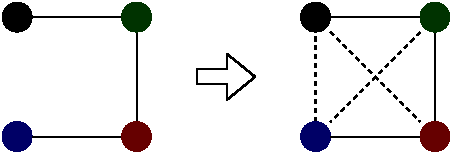
\includegraphics[scale = 0.9]{img/rid.pdf}
  \caption{Esempio di riduzione da ciclo hamiltoniano a TSP, con archi
    tratteggiati di peso 2 e archi normali di peso 1. Il colore dei vertici
    specifica che dalle due parti della trasformazione si ha lo stesso vertice}
  \label{fig:htsp}
\end{figure}
Controlliamo quindi i tempi. Voglio un costo della riduzione polinomiale e si ha
che l'aggiunta di archi, pesi e bound sono operazioni polinomiali.
\begin{definizione}
  Un problema $B$ è più difficile di un problema $A$, che ha in input la stringa
  $x$, sse:
  \[A\to B\]
  infatti ho:
  \[T(A(x))\leq F(x)+T(B(x))\]
\end{definizione}
\begin{definizione}
  Definiamo formalmente riduzione polinomiale tra un linguaggio $L_1$ e un
  linguaggio $L_2$ come:
  \[f:\Sigma_1^*\to \Sigma_2^*\]
  tale che:
  \[x\in L_1\iff f(x)\in L_2\]
  con $f$ calcolabile in tempo polinomiale ($O(|x|)$) dalla DTM. SI ha quindi
  che:
  \[L_1<_T L_2\]
\end{definizione}
\begin{definizione}
  Se si ha che $L_1<_T L_2$ e si ha che $L_2\in P$ allora sicuramente $L_1\in
  P$.\\
  Se avessi avuto $L_2\in NP$ o $L_2\not\in P$ non avrei informazioni su $L_1$. 

\end{definizione}
\begin{proof}
  Infatti e esiste un algoritmo polinomiale per $L_2$ allora, avendo una
  trasformazione polinomiale  ho che $f(x)+L_2$ è ancora polinomiale.
\end{proof}
\begin{definizione}
  Se si ha che $L_1<_T L_2$ e si ha che $L_1\not\in P$ allora ho che
  $L_2\not\in P$.
\end{definizione}
\begin{proof}
  Basta vedere ``al contrario'' il definizione precedente.
\end{proof}
Le riduzioni godono di proprietà:
\begin{itemize}
  \item riflessiva, $A\to A$
  \item transitiva, $A\to B\,\,\,\land \,\,\,B\to C\implies A\to C$, che essendo
  due trasformazioni in tempo polinomiale avrò comunque una trasformazione
  polinomiale 
\end{itemize}
Le riduzioni polinomiali \textbf{non sono sempre simmetriche} e quindi non sono
una relazione di equivalenza.\\
Abbiamo però una classe di equivalenza interna ai problemi NP, dove i problemi
contenuti sono i più difficili di NP e si riducono l'uno all'altro. Tali
problemi sono i problemi \textbf{NP-complete}.
\begin{definizione}
  Un linguaggio è \textbf{NP-complete} sse:
  \begin{itemize}
    \item $L\in NP$
    \item $L'<_TL,\forall\,L'\in NP$, tutti i linguaggi in NP si riducono a
    $L\in NP-complete$ e quindi i problemi in $NP-complete$ sono i più difficili
    di $NP$
  \end{itemize}
  Se ne risolvessi uno in tempo polinomiale risolverei tutti i problemi in NP in
  tempo polinomiale (ma ormai è assunto che non possa succedere anche se non si
  può dimostrare).
\end{definizione}
\begin{definizione}
  Ho che $P=NP$ sse esiste un linguaggio $L$ tale che:
  \[L\in NP-complete\cap P\]
\end{definizione}
\begin{proof}
  Se $P=NP$ allora sappiamo già che sarebbero polinomiali.\\
  Per l'altro verso ho che:
  \[\forall L'\in N, \,\,L<_T L\]
  e quindi esisterebbe un algoritmo polinomiale che risolve L per una DTM e
  quindi avrei un algoritmo polinomiale per ogni $L'\in NP$ per una DTM.
\end{proof}
Quindi se trovassi un algoritmo polinomiale per un NP-complete lo avrei per
tutti gli NP.
\begin{definizione}
  Se esiste un $L\in NP$ ma $L\not\in P$ allora:
  \[\forall L''\in \mbox{NP-complete}\]
  ho che $L''\not\in P$.
\end{definizione}
Dimostrando quindi che $P\neq NP$.\\
Andrebbe benissimo avere le prove di una di queste due situazioni, ma non esiste
ancora.\\
Per gli NP-complete vale anche la simmetria in quanto ogni problema NP-complete
è riducibile ad ogni altro problema NP-complete. Riprendendo l'esempio sopra so
che ciclo hamiltoniano è TSP, anche nelle forme decisionali, e quindi so che TSP
decisionale è NP-complete. La difficoltà è trovare almeno un problema
NP-complete, poi saprò che ogni altro a cui posso ridurlo è NP-complete.\\
Conosciamo moltissimi problemi NP-complete, molti riconosciuti tramite riduzioni
ma il primo è ottenuto tramite il \textbf{definizione di Cook}:
\begin{definizione}[definizione di Cook]
  SAT (che è stato già definito), che richiede un assegnamento di verità sulla
  formula $\phi$ in base all'assegnamento delle variabili $x_1,\ldots,x_n$, è
  NP-complete. 
\end{definizione}
\begin{proof}
  La dimostrazione completa è complessa ma vediamo qualche spunto.\\
  Si ha che SAT può essere risolto in tempo esponenziale, $O(2^n)$, provando
  tutti i possibili assegnamenti di verità possibili.\\
  Posso usare inoltre una NDTM che fa tutti i rami in parallelo, con ogni
  possibilità di assegnamento fatta in un ramo oppure posso dire che ``spara''
  un assegnamento a caso, che si suppone giusto, su un ramo e verifica che è
  giusto. In ogni caso con una NDTM avrei tempo polinomiale, $O(n\cdot m)$ per
  $n$ variabili e $m$ clausole.\\
  Per vedere che ogni problema NP, per semplicità decisionali, si riduce a SAT
  vedo che tutti i problemi in NP hanno in comune di avere un NDTM che li
  risolve in tempo polinomiale, che decide il linguaggio associato. Basta quindi
  dire che $\forall\Pi'\in NP$ ha associato una NDTM $N_\Pi'$ che lavora in
  tempo polinomiale e mi basta vedere che ogni NDTM che lavora in tempo
  polinomiale si può trasformare in una formula CNF, presa in ingresso da SAT,
  sfruttando poi gli stati finali della computazione di SAT. Se SAT dice che è
  soddisfacibile allora lo è il problema iniziale e quindi il problema è
  riducibile a SAT.
\end{proof}
SAT è stato il primo problema identificato come NP-complete ed è stato usato per
riconoscere gli altri problemi NP-complete.\\
La descrizione di una NDTM deve quindi corrispondere ad una $\phi$ di SAT per
far vedere che tutti i problemi NP si riducono a SAT. Si avrà una variabile per
ogni stato, una variabile per ogni carattere e una variabile per la posizione
della testina. Queste variabili saranno quelle che comporranno la $\phi$ e il
loro assegnamento comporterà la veridicità della formula.\\
Bisogna far vedere che $SAT<_T \Pi$ per far vedere che $\Pi$ è
NP-complete. Facendo poi vedere che un altro problema si riduce a $\Pi$ o SAT
dimostro che anche questo secondo problema è NP-complete. \\
Si ha che il problema del ciclo hamiltoniano e TSP, decisionali, siano
NP-complete.\\
Vediamo che $SAT<_T 3SAT$, che ha tre letterali in ogni clausola. Ho in input
una formula $\phi$ che deve diventare una $\phi_3$ tale che $\phi$ è
soddisfacibile sse $\phi_3$ lo è. La formula $\phi$ ha tante clausole in
congiunzione tra loro con un numero arbitrario di letterali ma $\phi_3$ deve
averne altrettante ma con soli tre letterali per clausola. Qualora si abbiano
clausole in $\phi$ con un solo letterale si aggiungono due letterali (che
indichiamo con $z$) in modo
però che la veridicità sia basata solo sulla variabile iniziale (questo vale per
tutte le trasformazioni che stiamo per mostrare, ovvero la veridicità deve
valere in base solo alle variabili iniziali della formula $\phi$). Tale clausola
che conteneva solo $x_1$ diventa una quadrupla clausola:
\[(x_1\lor z_1\lor z_2)\land (x_1\lor\neg z_1\lor z_2)\land (x_1\lor z_1\lor\neg
  z_2)\land(x_1\lor\neg z_1\lor\neg z_2)\] 
Se invece avessi una formula con due letterali diventa, aggiungendo una sola
variabile: 
\[(x_1\lor x_2\lor z_1)\land (x_1\lor x_2\lor \neg z_1)\]
Una formula a tre letterali resta ovviamente invariata mentre quelle a più
letterali vanno spezzate (aggiungendo poi variabili). Per esempio, avendo
quattro letterali, otterrei:
\[(x_1\lor x_2\lor z_1)\land (\neg z_1\lor x_3\lor z_2)\land (\neg z_2\lor
  x_4\lor z_3)\land\cdots\land(z_{n-3}\lor x_{n-1}\lor x_n)\]
Si vede che ogni formula di SAT può essere trasformata in una di 3SAT e quindi
anche quest'ultimo è NP-complete. Si dimostra che invece 2SAT non è NP-complete
ma ogni $K$SAT, con $K>2$, è NP-complete.\\
Anche, per esempio, il \textit{problema della colorabilità} è NP-complete, in
quanto può essere ridotto a SAT (non vedremo come).\\
Torniamo a parlare di TSP, non di decisione. Ho capito che serve tempo
esponenziale per risolverlo quindi si può pensare che sia NP-complete. Passo
quindi alla versione di decisione. Vedo però che ciclo
hamiltoniano, che è NP-complete, si riduce a TSP decisionale che quindi è
anch'esso NP-complete. Abbiamo comunque che TSP è più difficile del suo problema
decisionale, infatti D-TSP si riduce a TSP. Si ha quindi che TSP è
\textbf{NP-hard}, ovvero tutti i problemi NP si riducono ad esso ma il problema
stesso non è in NP (essendo un problema di ottimo e quindi non gli posso
associare un linguaggio) e quindi non è NP-complete (non essendo in NP). Per
TSP servirebbe una \textbf{macchina di Turing ad oracolo}.
\subsection{Rapporto spazio e tempo}
Aggiungiamo qualcosa a quanto già detto nelle sezioni precedenti.\\
\begin{definizione}
  Definisco la \textbf{funzione di complessità spaziale} come:
  \[f:\mathbb{N}\to\mathbb{N}\]
  con $f(n)$ che è il massimo numero di caselle utilizzate da una TM per
  decidere un certo linguaggio $L$ tutte le istanze di una certa dimensione,
  $n=|x|$. 
\end{definizione}
Sappiamo che, dal punto di vista del tempo (in notazione si ha $dtime=time$):
\[P=\bigcup_{k\geq 1}dtime(n^k)\]
\[NP=\bigcup_{k\geq 1}ntime(n^k)\]
\begin{definizione}
  Definiamo la \textbf{classe DSPACE} come l'insieme di tutti i linguaggi tali
  che sono decisi da una TM in spazio $O(f(n))$. Si ha che;
  \[PSPACE=\bigcup_{k\geq 1}dspace(n^k)\]
  avendo quindi limite polinomiale.
\end{definizione}
\begin{definizione}
  Definiamo la \textbf{classe NSPACE} come l'insieme di tutti i linguaggi tali
  che sono decisi da una NDTM in spazio $O(f(n))$. Si ha che:
  \[NPSPACE=\bigcup_{k\geq 1}nspace(n^k)\]
  avendo quindi limite polinomiale.
\end{definizione}
Come vale:
\[P\subseteq NP\]
Vale che:
\[PSPACE\subseteq NPSPACE\]
e per dimostrarlo mi concerto su una macchina che si preoccupa solo dello spazio
e non del tempo.\\
Prendiamo nuovamente il problema SAT e quindi ragioniamo sulla NDTM. Vediamo che
SAT è in NPSPACE per ovvi motivi (capisco che ramo scegliere e tale ramo ha una
casella per letterale, avendo spazio $n$) ma vediamo se appartiene anche a
PSPACE. Una DTM potrebbe provare tutte le possibilità in tempo esponenziale ma
in spazio polinomiale in quanto si sovrascrivono ad ogni tentativo le varie
caselle indicanti gli assegnamenti di verità ma la cardinalità di tali caselle è
sempre la stessa, una per ogni letterale, ovvero $n$. Quindi ho che $SAT\in
PSPACE$ anche se non è un'informazione così eclatante a causa del tempo
esponenziale.
\begin{definizione}[definizione di Savitch]
  Si dimostra che:
  \[PSPACE=NSPACE\]
  Quindi la DTM e la NDTM hanno la stessa potenza dal punto di vista dello
  spazio di calcolo.
\end{definizione}
\begin{proof}
  Un problema abbiamo visto essere definito come \textbf{configurazione
    raggiungibile}, ovvero se una macchina può andare da una configurazione
  iniziale $c_i$ ad una finale $c_f$ in un certo numero di passi $t$, indicato
  con:
  \[(c_i,C_f,t)\]
  Prendo una
  configurazione intermedi $c_m$ e vedo se vale:
  \[\left(c_i,C_m,\frac{t}{2}\right)\land \left(c_m,C_f,\frac{t}{2}\right)\]
  Spezzo poi in modo D\&I di volta in volta, vedendo ricorsivamente se entrambi
  i rami sono validi.\\
  Vedo che lo stack delle chiamate ricorsive ha una certa profondità. Una NDTM
  andrebbe in spazio $f(n)$ ha associata una DTM che lavora in spazio
  $O(f^2(n))$ in quanto salvo le varie configurazioni dello stack ricorsivo,
  avendo $2^{\log f(n)}=f(n)$.\\
  (\textbf{rivedere tutta la dimostrazione, quanto scritto è errato in buona
    parte!})
  
\end{proof}
Abbiamo quindi $PSPACE=NPSPACE$ e che $P\subseteq NP$ quindi certamente:
\[P\subseteq PSPACE\]
\[NP\subseteq NPSPACE\]
Si ha quindi la figura \ref{fig:cla}.
\begin{figure}
  \centering
  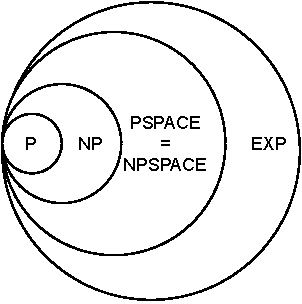
\includegraphics[scale = 0.9]{img/cla.pdf}
  \caption{Diagramma di Venn delle classi fin'ora descritte}
  \label{fig:cla}
\end{figure}
Abbiamo anche le classi $CO\_P$ e $CO\_NP$ ovvero le classi dei problemi
complementari $P$ e $NP$. Si ha che, a causa del determinismo:
\[CO\_P=P\]
ma quando si introduce il non determinismo le cose cambiano. La domanda iniziale
era del tipo \textit{esiste almeno uno} quindi il completamento è \textit{non
  esiste nessuno}, quindi devo verificare tutti i casi, andando in un caso che
nemmeno la NDTM riesce a risolvere, si finisce infatti nella classe
$EXP$. Quindi si ha che:
\[P\subseteq CP\_NP\land P\subseteq NP\]
non avendo un rapporto diretto e definito tra $NP$ e $CO\_NP$.

